\begin{problem}{XOR}{стандартный ввод}{стандартный вывод}{3 секунды}{256 мегабайт}

Даны $n$ прямоугольников левый нижний угол которых находится в $(0, 0)$, а правый верхний в $(i, A_i)$. Гарантируется, что $A_{i}$ не возрастают

Площадью симметрической разности двух прямоугольников назовем площадь, которая покрывается одним или другим прямоугольником, но не обоими сразу.

Нужно находить два прямоугольника $i$, $j$, такие что $l \leq i < j \leq r$, а площадь симметрической разности максимальна

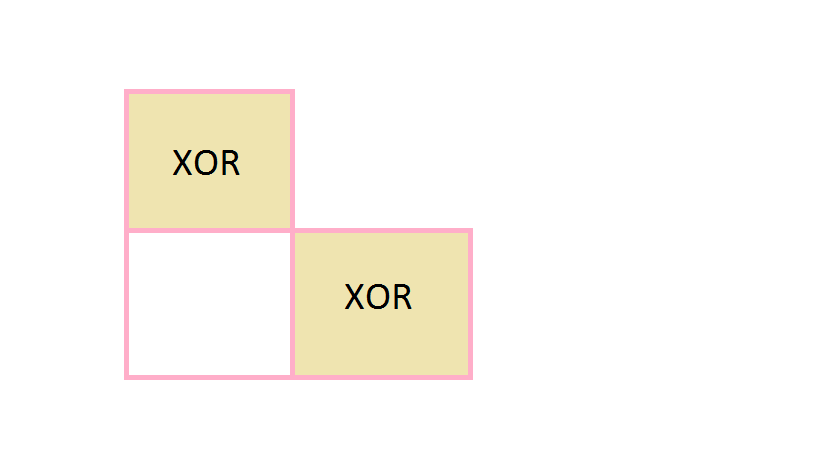
\includegraphics[width=18cm, height=10cm]{picture.png}

\InputFile
В первой строке записано целое число $n$ ($2 \le n \le 100\,000$) ~--- количество прямоугольников.

Во второй строке записано $n$ чисел, для каждого $i$ $(1 \le i \le n)$ $i$-е обозначает $A_{i}$ ($1 \le A_{i} \le 10^9$, $A_{i} \ge A_{i + 1}$).

В следующей строке записано целое число $q$ ($1 \le q \le 100\,000$) ~--- количество запросов.

В последующих $q$ строках вводятся $l_{i}, r_{i}$ $(1 \le l_{i} < r_{i} \le n)$

\OutputFile
На каждый запрос вывести максимальную площадь симметрической разности двух прямоугольников на отрезке.

\Example

\begin{example}
\exmp{7
10 9 9 8 8 6 6
4
2 7
1 3
4 5
3 6
}{36 19 8 27 }%
\end{example}

\end{problem}

